\documentclass[conference]{IEEEtran}
\IEEEoverridecommandlockouts
% The preceding line is only needed to identify funding in the first footnote. If that is unneeded, please comment it out.
\usepackage{cite}
\usepackage{amsmath,amssymb,amsfonts}
\usepackage{algorithmic}
\usepackage{graphicx}
\usepackage{textcomp}
\usepackage{xcolor}
\bibliographystyle{ieeetr}
\newcommand{\etal}{\textit{et al.}}
\begin{document}

\title{Multimodal for Natural Language Processing: Tasks, Methodologies and Advancements\\
}

\author{\IEEEauthorblockN{M. Arsalan}
\IEEEauthorblockA{
\textit{MBZUAI}\\
Abu Dhabi, UAE \\}
\and
\IEEEauthorblockN{S. AlBarri}
\IEEEauthorblockA{
\textit{MBZUAI}\\
Abu Dhabi, UAE \\}
}

\maketitle

\begin{abstract}
Modality is derived from the word “mode”, which means the methodology of communicating or experiencing things. Artificial Intelligence (AI) mimics humans to understand the world around us by interpreting modality. The learning ability of deep neural networks uplifted AI performance in every domain. Natural Language Processing (NLP), which is an AI core application, progressed remarkably by learning semantic meaning and adapting contextual information of the text modality. Multimodal learning is the phenomenon where the essence of information is extricated from different modalities (text, image, audio, emotions, expressions) while maintaining correlation. This study presents NLP applications enhanced by multimodal data to train and make deep learning architecture more robust. The applications presented are visually rich document understanding, sentiment analysis, visual question answering, event and fake news detection, and information retrieval. For each application, recent studies, challenges,  SOTA deep learning architecture and benchmark datasets are presented.           
\end{abstract}
\begin{IEEEkeywords}
Multimodal Data, Natural Language Processing, deep learning, representation, speech, and vision. 

\end{IEEEkeywords}


\section{Introduction}
  From information retrieval to image processing, and from text mining to recommendation systems, the research community shifted to deep learning-based approaches for complex applications \cite{guo2019deep}. Although deep learning architecture imitate the behavior of the human brain's neurons, most of the previous research is performed considering unimodal data and learns one mode or source of information to build a machine learning application. However, for an AI model to mimic the human experience accurately and improve its performance, multimodalities play vital role \cite{wignell2021natural}. Multimodalities include a combination of two or more modes such as text, images, video, audio, speech, body gestures, facial expressions, physiological signals and voice tone \cite{recent_paper}.
 
 Multimodal machine learning is a complicated task as it entails many challenges, five central challenges are listed in \cite{baltruvsaitis2018multimodal}. The five challenges are representation \cite{bench1}, translation \cite{translation}, alignment, fusion \cite{fusion}, and co-learning \cite{co-learn}. Each challenge in multimodal applications by itself is the subject of an extensively researched field. Representation is the method by which raw data is summarized or \textit{represented}. For instance, physiological information, audio, and voice can be represented as signals, whereas, language such as typed text can be represented symbolically. To perform cross-modality signal processing, the multimodal signals need to be projected and represented into a single vector space. Translation is the process of transforming or \textit{translating} data from one modality to another. Translation showcases the subjectivity and open-endedness faced in representing a modality.  Alignment is the process of identifying relationships between or \textit{aligning} elements from two or more modalities. Dependencies and similarities between modalities are exploited in alignment to accomplish multimodal downstream tasks. Fusion integrates or \textit{fuses} information from two or more unimodal data to perform prediction tasks. Fusion leverages the rich features offered in each unimodal data to build multimodals for various downstream tasks. The input of fusion is the unimodal embedding or representations and the output is implemented for a multimodal task. Finally, co-learning transmits knowledge or \textit{learned} information between two or more different modalities or between their representations. The five challenges, as involved as they are, simplifies multimodal downstream tasks reality by assuming that all of the modalities are present, aligned, noiseless, and correctly and fully annotated during training and testing. Figure 1 comprehensively demonstrates the five challenge and the notion of transferring different unimodals into shared and common space.                      
 
 For the purpose of the proposal, multimodality applications in Natural language processing (NLP) are introduced. This proposal is divided as follows, in Section II, the Literature Review introduces previous attempts to summarize and survey multimodal application. In Section III, the Plan Forward defines and expands on various key multimodal applications. Finally, the conclusion summarizes the expected future work to build the survey paper.  
 The expected contributions of this survey are: 
 \begin{itemize} 
 \item Focus on main NLP tasks that can be performed efficiently using multimodality. 
    \item Expand on several multimodal applications, note their challenges, present SOTA architectures and benchmark datasets. 
    \item Reflect on the current literature and discuss possible improvement and future directions. 
 \end{itemize} 
\begin{figure*}
    \centering
  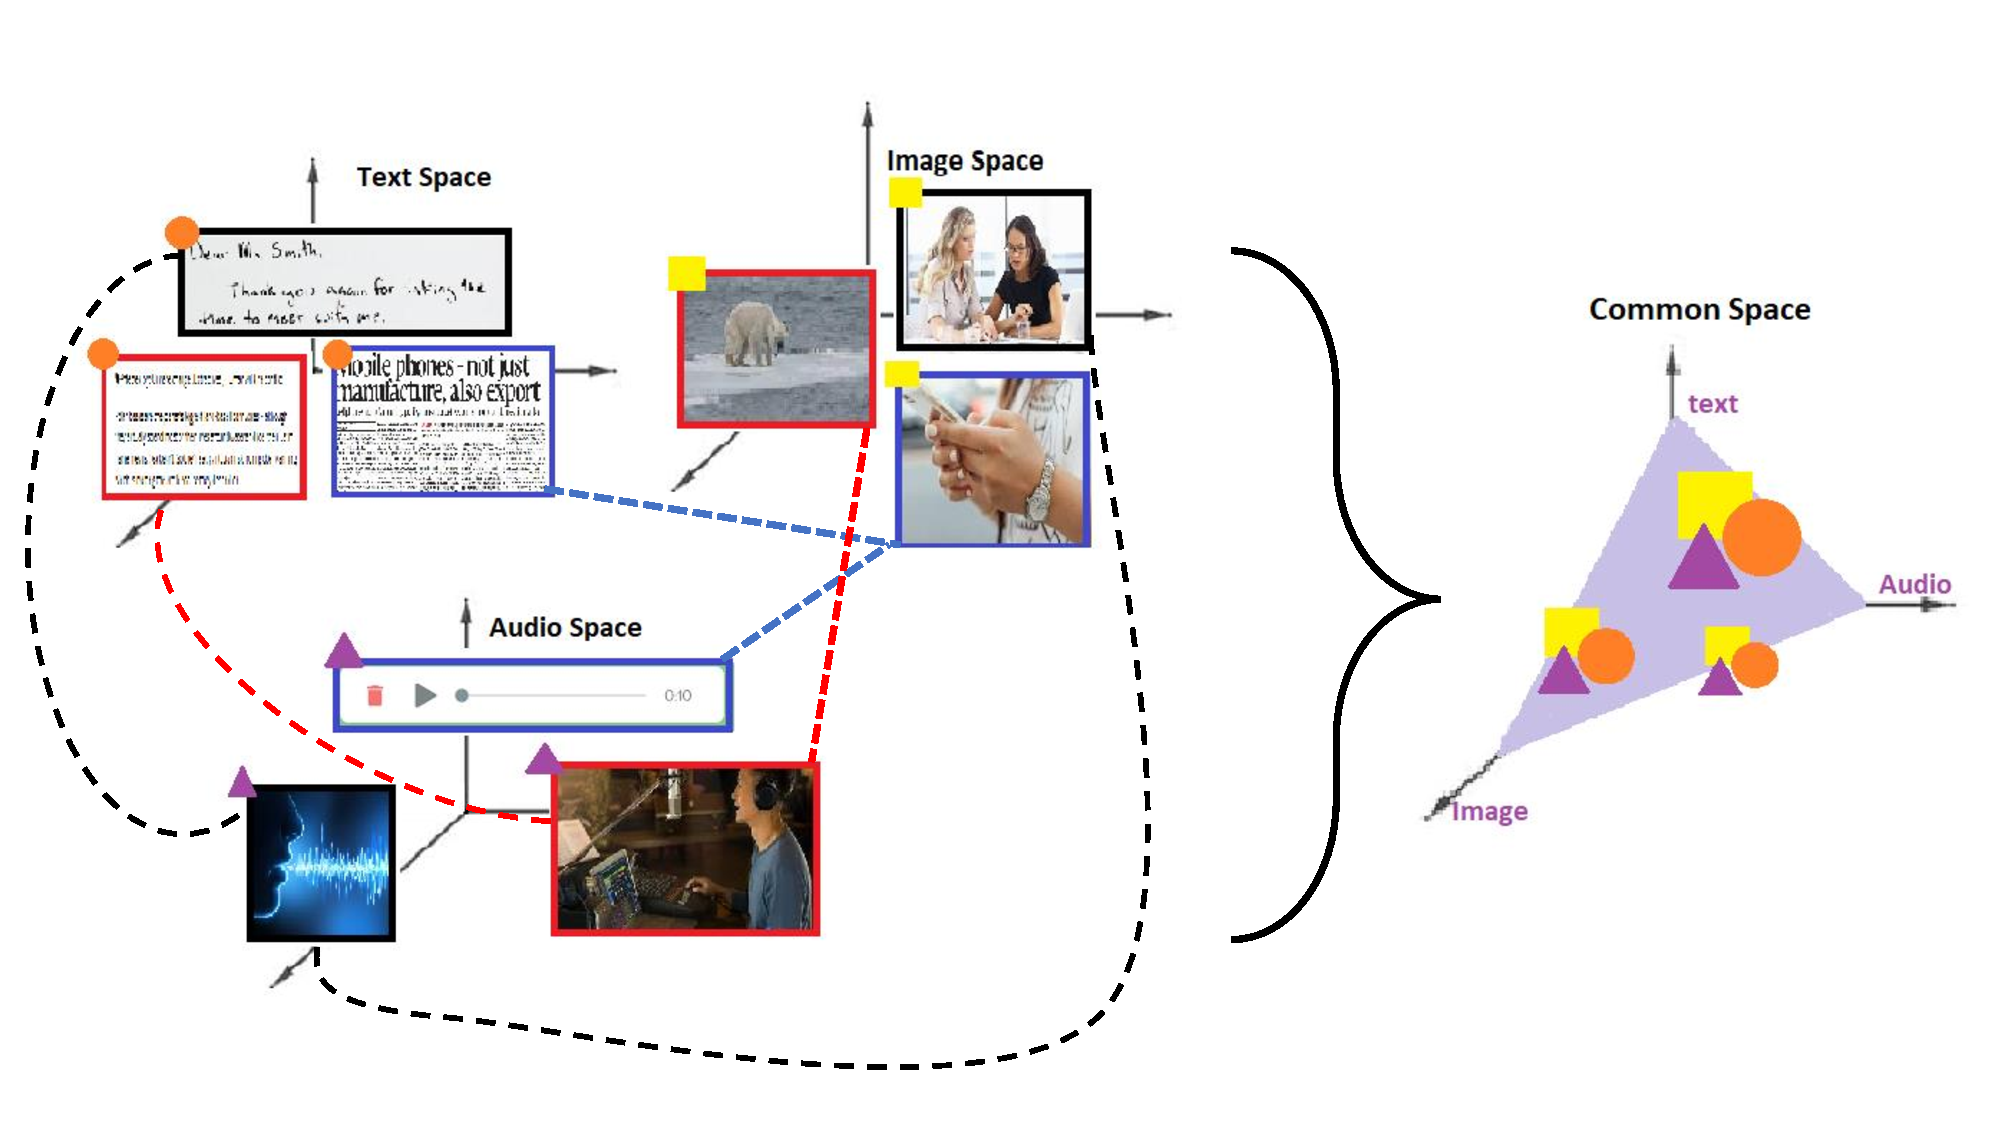
\includegraphics[width=14cm,height=6cm]{Presentation1.pdf}
  \caption{Text, images and audio modalities are represented using their own features and dimensions. In multimodal applications, text, images, and audio are jointed in a common representation. The common space integrates and maps the information from each modality. Common space representation is essential and detrimental in multimodal downstream tasks.}
\end{figure*}

\section{Literature Review}
Researchers got inspiration from the multimodal approach used for audio-visual speech recognition \cite{mcgurk1976hearing}. Well-aligned integration of vision and hearing was a fundamental requirement of the task. Results motivated the research community to extend this idea for other tasks. The multimodal approach evolved with time and has been used for different speech, vision and emotion recognition applications in the past \cite{baltruvsaitis2018multimodal}. The most recent category contains the data from multimedia resources that can be more complex than two or three modalities. The multimodal data brought up numerous applications that solve the problems more efficiently and creatively than unimodal data. 

The representative application is image captioning which generate the text description of the image. Document understanding \cite{im2021self} extract layout, visual features, table like structural information from the documents. Sentiment Analysis \cite{chandrasekaran2021multimodal} of reviews, tweets and posts containing Video, images, emojis and any other emotional expression. Detection includes the identification of the specific event, discovering trend, finding out emergency situation and detecting fake news on web or social media \cite{wang2022fmfn}. Information retrieval also rely on multimodal processing, especially in electronic health records, where the data related to patient is available in different modalities \cite{zhang2021learning}. 

The first challenge that algorithm face while dealing multimodal data is to understand the encoding information of different modalities which is called heterogeneity gap in learning Representation \cite{rasiwasia2010new}. The heterogeneity gap can be reduced by associating the similar semantic of different modalities in correlated manner. Fusing features from different modalities boosted the performance on cross media tasks \cite{habibian2016video2vec}.  

Recent research depicts that deep learning outperformed the classical approach in understanding and processing representation due to strong learning abilities \cite{lecun2015deep}. The key phenomenon is to learn representation in a hierarchical manner as general purpose learning without structural or additional information. Mentioned reasons flourished deep learning as most compatible approach for multimodal representation learning. 

Numerous surveys are published for deep learning multimodal detailing the applications of computer vision and Natural language processing \cite{ramachandram2017deep}. Various publications focus on multimodal representation, correlation, fusion, translation and co-learning \cite{guo2019deep}, \cite{baltruvsaitis2018multimodal}. Some authors focused on general application related to NLP and CV and few authors addressed single application using multimodal architecture \cite{stappen2021multimodal}, \cite{chandrasekaran2021multimodal}. Most of the previous work found is related to enhance the computer vision applications as textual features are semantically rich \cite{bayoudh2021survey}.  

In this study, effort is put to discuss Natural Language Processing tasks considering multimodal data. We aim to present a comprehensive survey that consider several modalities including text, images, speech, expressions, gestures and other signals. Additionally, variations of deep neural networks that are utilized to deal multimodal data under each application are discussed. Table 1 presentsbenchmark datasets and the modalities entailed for each application. 
 
\section{Plan Forward}
In this section, the taxonomy of the survey is proposed along with the subcategories of each application. All NLP applications that are enhanced by deep multimodal architectures are presented here. Details include for each multimodal application, its benchmark dataset in literature, evaluation metrics, description, and comparison for the best performing architectures. Multimodal applications are visually rich document understanding, sentiment analysis, event detection, information retrieval and processing, classification, dialogue systems, recognition, and cross-modality.      

\subsection{Visually Rich Document Understanding}
The understanding of documents that are visually rich and contain structured information is important to analyze business and market applications \cite{im2021self}. Contrary to the classical information extraction methods, Visually Rich Documents (VRD) understanding considers visual layout along with the text. One of the recent research, LayoutLMv2 \cite{xu2020layoutlmv2}  pre-trained the Transformer-based model that learns from different modalities at the pre-training stage by integrating and aligning layout, textual and visual information. LayoutMv2 used more than 10 billion documents to achieve pre-trained model that performed SOTA on document understanding tasks. More recently, Li \textit{et al.} \cite{li2021structext} proposed StrucTexT, which outperformed LayoutLMv2 by pre-training the Transformer model in a self-supervised manner, consumed less number of parameters, and achieved high scores. The publicly available benchmark datasets for downstream tasks are SROIE \cite{huang2019icdar2019}  and FUNSD \cite{jaume2019funsd}. LayoutLMv2 achieved 97\% and 84\% F1 score on SROIE and FUNSD, respectively. StrucTexT accomplished 96.88\% and 85.68\% F1 on SROIE and FUNSD, respectively.  


\subsection{Sentiment Analysis}
Sentiment analysis is the core task in NLP that extract and classify reviews, feeling, gestures and behavior toward specific entity. Sentiment Analysis understands people' perspectives for efficient decision making in multiple domains. Textual representation has been analysed widely in previous research such as \cite{kim2016topic}, \cite{camacho2017role}, and \cite{wood2021market}. However, sentiment analysis task moved from text modality only to other form of modalities due to social media and internet. Chen \textit{et al.} \cite{chen2020swafn} designed deep learning architecture to extract sentiment from multimodal complex data. The author proposed two component-based methods consisting of shallow fusion and aggregation parts. The shallow fusion component extracts contextual information from the different domains using the attention mechanism and the aggregation part attains sentimental word aware fusion. The proposed architecture outperformed other methods by achieving the highest score on benchmarks multimodal datasets CMU-MOSI, CMU-MOSEI, and YouTube datasets for sentiment analysis. 



\subsection{Visual Question Answering}
Visual Question Answering (VQA) attempts to answer linguistic questions by retrieving information from a visual cue \cite{VQA}. VQA combines information from understanding written questions and from focusing on the related information in the high dimensional visual. Questions could vary from a simple true/false to knowledge-based and open-ended questions, whereas visuals could vary from a simple sketch or image to a whole video. Furthermore, VQA simultaneously combines several functions from NLP and CV fields such as language understanding, relation extracting, attribute and object classifying, counting, knowledge-base and common-sense reasoning \cite{recent_paper}.  
VQA maps question text and visual embeddings obtained via recurrent and convolutional neural networks (RNN and CNN), respectively, to a common vector space. Mapping to the shared vector space enables VQA to tackle open-ended free-form questions. In the literature, the four general mapping approaches are joint embedding \cite{vqa_emb}, attention mechanism \cite{vqa_att}, compositional model \cite{vqa_comp} and knowledge base \cite{vqa_kb}.     
There exist review papers targeting VQA as a research field of its own such as in \cite{VQA} and \cite{VQA2}. In addition to surveys, benchmarks such as \cite{bench1} by Carnegie Mellon University (CMU) and \cite{bench2} are available. Benchmark datasets are VAQ v1.0 \cite{VQA2}, VAQ-X \cite{vqa-x}, and VAQ-CP \cite{vqa-cp}.    

\begin{table}[]
\caption{The NLP applications, Benchmark datasets and modalities are mentioned.}
\label{tab:my-table}
\begin{tabular}{|l|l|ll|}
\hline
\textbf{Applications}                                                           & \textbf{Benchmarks} & \multicolumn{2}{l|}{\textbf{Dataset Nature}} \\ \hline
\begin{tabular}[c]{@{}l@{}}Visually Rich \\ Document Understanding\end{tabular} & FUNSD               & \multicolumn{2}{l|}{Scanned Documents}       \\ \hline
Sentiment Analysis                                                              & CMU-MOSEI           & \multicolumn{2}{l|}{Videos + Sentences}      \\ \hline
Visual Question Answering                                                       & VQA v1.0            & \multicolumn{2}{l|}{Images + sentences}      \\ \hline
Event Detection                                                                 & CrisisMMD           & \multicolumn{2}{l|}{Tweets + Images}         \\ \hline
Fake News Detection                                                             & Weibao              & \multicolumn{2}{l|}{Images + sentences}      \\ \hline
Information Retrieval                                                           & MIMIC               & \multicolumn{1}{l|}{X-ray + Reports}    &    \\ \hline
\end{tabular}
\end{table}

\subsection{Event Detection}
 Detection of an event, trend or situation specifically through content available on social media become more efficient and generous by considering data from different modalities \cite{hu2017adaptive}. A massive amount of data is generated that has a significant impact on the lives, property, and psychology of humans \cite{algiriyage2022multi}.Event detection can be mapped to other realistic scenarios, such as Emergency management, Disaster Detection, and Topic Detection \cite{xiao2022survey}. The researchers are designing architectures to detect events using multimodal data that maintain comprehensive information. Even though the data from different perspectives enhance the performance, likewise,  the challenges are increased for methods to deal with redundant and heterogeneous characteristics.       
For disaster detection, still there is no large enough benchmark dataset is available to employ deep learning architecture except CrisisMMD \cite{alam2018crisismmd}, CrisisNLP and CrisisLex.
For traffic event detection, Chen \textit{et al.} \cite{chen2021multi} , created a multimodal dataset by integrating the traffic related filtered tweets with sensor data. The author achieved 84\%, 83\%, 87\% F1 score with CNN, RNN, and mmGAN (multimodal GAN) models, respectively.  

\subsection{Fake News Detection}
Fake news utilize multimedia information to cause the panic on social media. The version of content containing text and image misinterpret the facts and manipulate human psychology which can lead to rapid false propagation of fake news \cite{jin2017multimodal}. The multimodal architecture can detect fake news by mismatching the pattern and considering the similarity among different modalities \cite{zhou2020safe}.

Wang \textit{et al.} \cite{wang2022fmfn} proposed the fine-grained multimodal fusion networks (FMFN) to detect fake news detection in efficient way. The author presented their approach in following three steps. CNNs are used to extract visual featues and RoBERTa \cite{liu2019roberta} is used to attain contextualized embedding of words in the first step. In second phase, attention mechanism is used between visual and textual features to enhance the correlation for fusing features. At final stage, binary classifier adopted to perform detection on fused features.  
The author evaluated the proposed model on Weibao Dataset \cite{jin2017multimodal} by focusing only tweets that contains text and images. The proposed model acquired 88\% accuracy as compared to CARMN which scored 85\%.   


\subsection{Information Retrieval} 
To build an Information Retrieval (IR) application, the steps are indexing, query formulation, retrieval and evaluation. In indexing and query formulation, documents and user interfaced queries are represented by their characteristic features, respectively \cite{EHR}. The retrieval system then maps both representations to retrieve or extract the required useful information. The performance of the retrieval task is evaluated based on recall and precision. In multimodal information retrieval, the system searches documents with different modalities such as text, images, videos, or physiological signals and images. Employing more than one modality enriches information retrieving processes. One example of multimodal information retrieval is in electronic health records. 

\subsubsection{Electronic Health Records}
Patients health records contain various modalities such as categorical data, text, images such MRI scans, or signals such as electrocardiogram (ECG) \cite{EHR}. Information retrieval system can extract information from different modalities to report, present, and/ or predict a patient health status. For instance, Supervised Deep Patient Representation Learning Framework (SDPRL) engages different modalities information to learn patient representation \cite{zhang2021learning}. SDPRL is build and tested using the benchmark  dataset MIMIC-III. 



\section{Conclusion}
% Add more application -cross modality 

% details added 
% challenges for each application on Fusion representation,... level. 
% SOTA architecture for each application is explained  
The preliminary work for the literature review is proposed. The planned future trajectory is to add additional NLP multimodal applications such as machine translation, audio-visual speech recognition tasks, information processing, and cross-modality. Moreover, further details will be presented on the NLP applications by discussing the difficulties encountered in multimodal data representation, translation, alignment, fusion, and co-learning tasks. The SOTA architectures for each application are to be presented and detailed along with the performance, available benchmarks, and benchmark datasets. Results summary for different architectures will be tabulated to enhance the information reach and condensation in literature reviews  

\bibliography{references} 
\end{document}
